\documentclass{article}
\usepackage{amsmath}
\usepackage{amssymb}
\usepackage{graphicx}
\usepackage{mathtools}
\usepackage[margin=0.7in]{geometry}


\title{MAST30027 Modern Applied Statistics Assignment 4}
\author{Patrick Tjahjadi (890003)}
\date{Tutor: Qiuyi Li | Tutorial: Monday 12:00 PM}

\begin{document}


\pagenumbering{gobble}
\maketitle

\section{Question One}
f(x\textsubscript{i}) = $\frac{\sqrt{\tau}}{\sqrt{2\pi}}$\textit{e}\textsuperscript{-$\frac{\tau(x-\mu)\textsuperscript{2}}{2}$}\\
$\propto$ \textit{e}\textsuperscript{-$\frac{\tau(x-\mu)\textsuperscript{2}}{2}$}\\
$\implies$  f(x\textsubscript{1}, ..., x\textsubscript{100} $\vert$ $\mu$, $\tau$) $\propto$ $\prod_{i=1}^{n} e\textsuperscript{-$\frac{\tau(x-\mu)\textsuperscript{2}}{2}$}$ where n = 100\\

\subsection{Part A}
f($\tau$, $\mu$, x\textsubscript{1}, ..., x\textsubscript{100}) = f(x\textsubscript{1}, ..., x\textsubscript{100} $\vert$ $\mu$, $\tau$) p($\tau$, $\mu$)\\
$\propto$ $\prod_{i=1}^{n} (e\textsuperscript{-$\frac{\tau(x-\mu)\textsuperscript{2}}{2}$})$ ($\tau$)\textsuperscript{-1}\\\\
p($\mu$ $\vert$ $\tau$, x\textsubscript{1}, ..., x\textsubscript{100}) = $\frac{f(\mu, \tau, x\textsubscript{1}, ..., x\textsubscript{100})}{f(\tau, x\textsubscript{1}, ..., x\textsubscript{100})}$\\
$\propto$ f($\mu$, $\tau$, x\textsubscript{1}, ..., x\textsubscript{100})\\
$\propto$ $\prod_{i=1}^{n} (e\textsuperscript{-$\frac{\tau(x-\mu)\textsuperscript{2}}{2}$})$ ($\tau$)\textsuperscript{-1}\\
$\propto$ \textit{e}\textsuperscript{-$\sum_{i=1}^{n} (\frac{\tau}{2}(x\textsubscript{i} - \mu)\textsuperscript{2})$}\\
= \textit{e}\textsuperscript{-$\sum_{i=1}^{n} (\frac{\tau}{2}(x\textsubscript{i}\textsuperscript{2} - 2\mu x\textsubscript{i} + \mu\textsuperscript{2})$}\\
Given that $\sum_{}^{}x\textsubscript{i}$ = n$\bar{x}$,\\
= \textit{e}\textsuperscript{-$\sum_{i=1}^{n} (\frac{\tau}{2}x\textsubscript{i}\textsuperscript{2})$} \textit{e}\textsuperscript{-(-2$\mu$n$\bar{x}$ + n$\mu$\textsuperscript{2})$\frac{\tau}{2}$}\\
= \textit{e}\textsuperscript{-$\sum_{i=1}^{n} (\frac{\tau}{2}x\textsubscript{i}\textsuperscript{2})$} \textit{e}\textsuperscript{n(2$\mu$$\bar{x}$ - $\mu$\textsuperscript{2})$\frac{\tau}{2}$}\\
= \textit{e}\textsuperscript{-$\sum_{i=1}^{n} (\frac{\tau}{2}x\textsubscript{i}\textsuperscript{2})$} \textit{e}\textsuperscript{n(2$\mu$$\bar{x}$ - $\mu$\textsuperscript{2} + $\bar{x}$\textsuperscript{2} - $\bar{x}$\textsuperscript{2})$\frac{\tau}{2}$}\\
=  \textit{e}\textsuperscript{-$\sum_{i=1}^{n} (\frac{\tau}{2}x\textsubscript{i}\textsuperscript{2})$} \textit{e}\textsuperscript{n(2$\mu$$\bar{x}$ - $\mu$\textsuperscript{2} - $\bar{x}$\textsuperscript{2})$\frac{\tau}{2}$} \textit{e}\textsuperscript{$\bar{x}$\textsuperscript{2}$\frac{\tau}{2}$}\\
$\propto$ \textit{e}\textsuperscript{n(2$\mu$$\bar{x}$ - $\mu$\textsuperscript{2} - $\bar{x}$\textsuperscript{2})$\frac{\tau}{2}$} \\
=  \textit{e}\textsuperscript{-n($\bar{x}$ + $\mu$)\textsuperscript{2}$\frac{\tau}{2}$}\\
= \textit{e}\textsuperscript{-$\frac{(\mu - \bar{x}\textsuperscript{2})}{2\frac{1}{\tau n}}$}\\\\
This belongs to a normal distribution with mean $\bar{x}$ and variance $\frac{1}{\tau n}$.\\\\\\
p($\tau$ $\vert$ $\mu$, x\textsubscript{1}, ..., x\textsubscript{100}) = $\frac{f(\mu, \tau, x\textsubscript{1}, ..., x\textsubscript{100})}{f(\mu, x\textsubscript{1}, ..., x\textsubscript{100})}$\\
$\propto$ f($\mu$, $\tau$, x\textsubscript{1}, ..., x\textsubscript{100})\\
$\propto$ $\prod_{i=1}^{n} (\sqrt{\tau}e\textsuperscript{-$\frac{\tau(x-\mu)\textsuperscript{2}}{2}$})$ ($\tau$)\textsuperscript{-1}\\
= $\tau$\textsuperscript{$\frac{n}{2}$}\textit{e}\textsuperscript{-$\tau$$\sum_{i=1}^{n} (\frac{1}{2}(x\textsubscript{i} - \mu)\textsuperscript{2})$} ($\tau$)\textsuperscript{-1}\\
= $\tau$\textsuperscript{($\frac{n}{2}$-1)}\textit{e}\textsuperscript{-$\tau$$\sum_{i=1}^{n} (\frac{1}{2}(x\textsubscript{i} - \mu)\textsuperscript{2})$}\\\\
This belongs to a gamma distribution with shape $\frac{n}{2}$ and rate $\sum_{i=1}^{n} (\frac{1}{2}(x\textsubscript{i} - \mu)\textsuperscript{2})$.\\

\subsection{Part B}
A code that uses Gibbs sampling is derived from Heejung Shim's simulation\_Gibbs.pdf. The code is as follows:\\
\begin{center}
\includegraphics{1bcode}\\
\end{center}
1000 samples is performed for this simulation. Notice that no burn-in is used in this code.\\
Here, gibbs1 has inital values that are significantly higher than the actual values while gibbs2 has initial values that are significantly lower. The graph for mu becomes:\\
\begin{center}
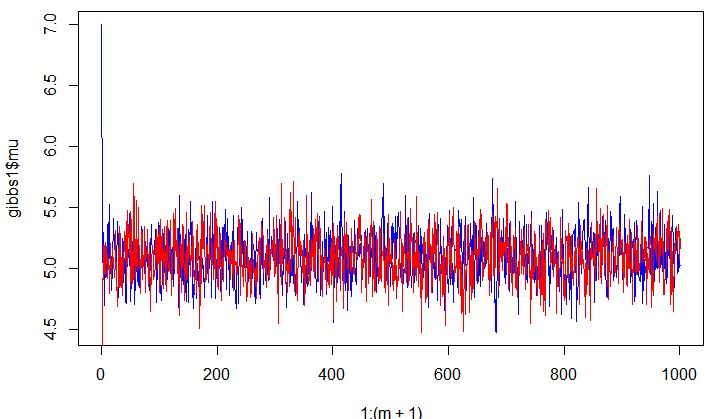
\includegraphics{1bgraphmu}\\
\end{center}
The graph for tau becomes:\\
\begin{center}
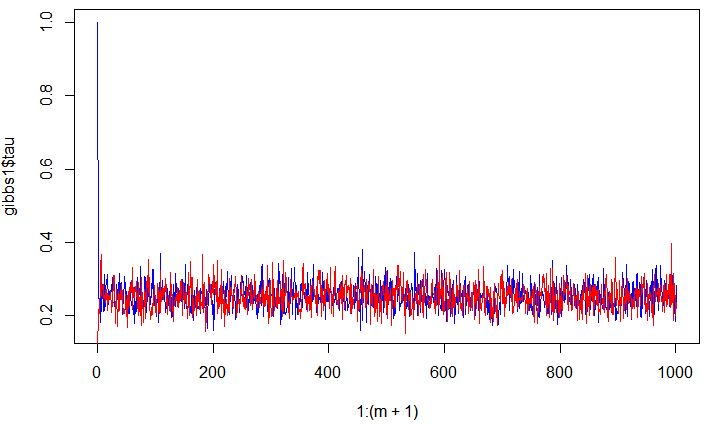
\includegraphics{1bgraphtau}\\
\end{center}
We can see that the Gibbs samples converge to approximately the actual values after a few samples for both chains. Hence, these samples from two different chains are mixed well and behave similarly.

\subsection{Part C}
The code is as follows:\\
\begin{center}
\includegraphics{1ccode}
\end{center}
Plotting the marginal posterior distributions yield the following graphs:\\
\begin{center}
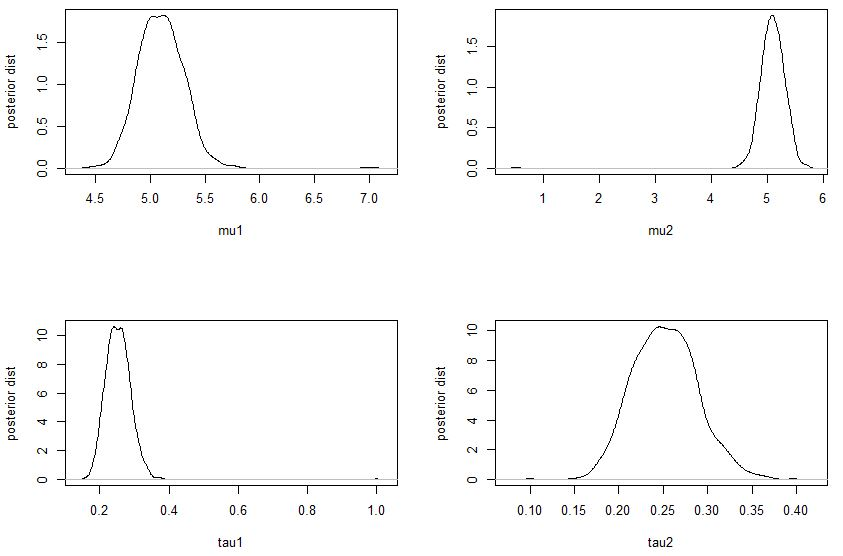
\includegraphics{1cgraph}
\end{center}
The marginal posterior means and credible intervals are:\\
\begin{center}
\includegraphics{1cstats}
\end{center}
This shows that the 95\% credible interval for mu is approximately (4.77, 5.42) and the 95\% credible interval for tau is approximately (0.199, 0.312).\\

\section{Question Two}
To determine the acceptance probability for this algorithm:\\
We are simulating Normal($\mu$\textsubscript{c}, $\tau$\textsubscript{n}) for $\mu$ and Gamma(5$\tau$\textsubscript{c}, 5) for $\tau$.\\
The proposed function Q will be symmetric, so we will be implementing a Random Walk MH algorithm:\\
\begin{center}
A (Acceptance Probability) = min(1, $\frac{\pi(\theta ')}{\pi(\theta)}$) = min(1, $\frac{\pi(\mu ', \tau ')}{\pi(\mu, \tau)}$)\\
\end{center}
$\pi$($\mu$', $\tau$') = f($\mu$, $\tau$, x\textsubscript{1}, ..., x\textsubscript{100})\\
= p($\tau$', $\mu$') * p(x\textsubscript{1}, ..., x\textsubscript{100} $\vert$ $\mu$', $\tau$')\\\\
$\implies$ log$\pi$($\mu$', $\tau$') = log p($\tau$', $\mu$') + log p(x\textsubscript{1}, ..., x\textsubscript{100} $\vert$ $\mu$', $\tau$')\\
$\propto$ log($\frac{1}{\tau '}$) + $\sum_{i=1}^{n} log(p(x\textsubscript{i} \vert \mu  ', \tau'))$\\\\
$\implies$ $\pi$($\mu$', $\tau$') = \textit{e}\textsuperscript{(log$\frac{1}{\tau '}$) + $\sum_{i=1}^{n} log(p(x\textsubscript{i} \vert \mu  ', \tau'))$} and $\pi$($\mu$, $\tau$) = \textit{e}\textsuperscript{(log$\frac{1}{\tau}$) + $\sum_{i=1}^{n} log(p(x\textsubscript{i} \vert \mu, \tau))$}\\\\
$\therefore$ A = min(1, $\frac{\textit{e}\textsuperscript{(log$\frac{1}{\tau '}$) + $\sum_{i=1}^{n} log(p(x\textsubscript{i} \vert \mu  ', \tau'))$}
}{\textit{e}\textsuperscript{(log$\frac{1}{\tau}$) + $\sum_{i=1}^{n} log(p(x\textsubscript{i} \vert \mu, \tau))$}}$)




\subsection{Part A}
The code to run the MH algorithm is as follows:
\begin{center}
\includegraphics{2acode1}\\
\includegraphics{2acode2}\\
\end{center}
10000 iterations are performed with 2 chains. Note that chain[,1] refers to mu while chain[,2] refers to tau. The initial values are set the same as for the Gibbs sampling to see how they compare. Here, "chain" has initial values that are significantly higher than the actual values while "chain2" has initial values that are significantly lower. The graph for mu becomes:\\
\begin{center}
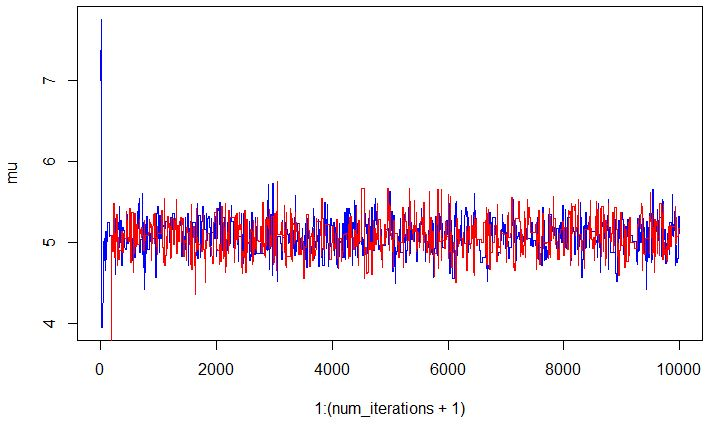
\includegraphics{2agraphmu}\\
\end{center}
The graph for tau becomes:\\
\begin{center}
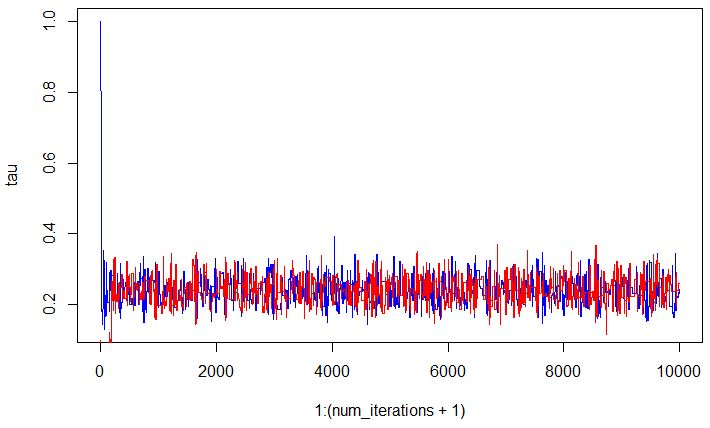
\includegraphics{2agraphtau}\\
\end{center}
We can see that the MH algorithm samples also converge to approximately the actual values after a few samples for both chains. Therefore, it can also be inferred that these samples from two different chains are mixed well and behave similarly.

\subsection{Part B}
Similar to question 1C, the code is as follows:\\
\begin{center}
\includegraphics{2bcode}
\end{center}
Plotting the marginal posterior distributions yield the following graphs:\\
\begin{center}
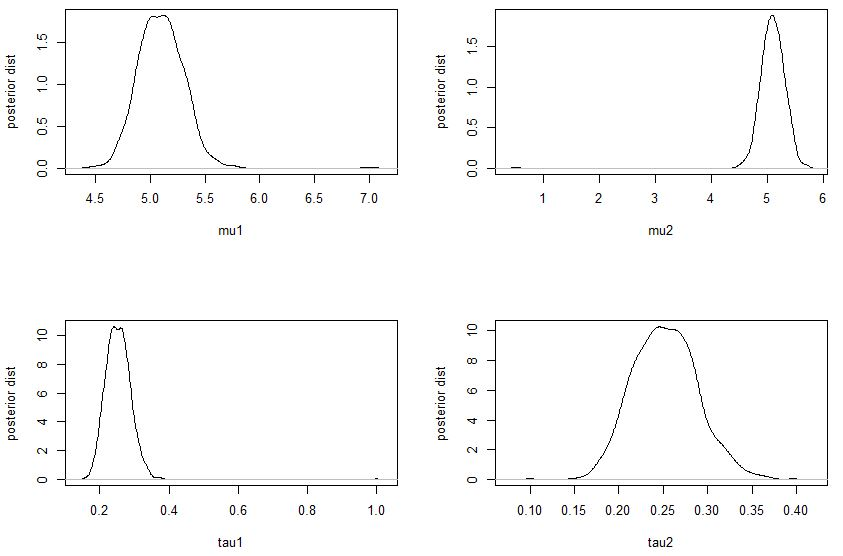
\includegraphics{1cgraph}
\end{center}
The marginal posterior means and credible intervals are:\\
\begin{center}
\includegraphics{2bstats}
\end{center}
This shows that the 95\% credible interval for mu is approximately (4.77, 5.41) and the 95\% credible interval for tau is approximately (0.188, 0.302).\\

\end{document}